\documentclass[polish, a4paper, 12pt, oneside]{book}
\linespread{1.3}
\usepackage[a4paper, inner=0cm, outer=0cm, top=2.7cm, right=2.4cm, bottom=2.5cm, left=2.4cm, bindingoffset=1.2cm]{geometry}
\usepackage[utf8]{inputenc}
\usepackage[T1]{fontenc}
\usepackage{lmodern}
\usepackage{microtype}
\usepackage{graphicx}
\usepackage{index}
\usepackage{babel}
\usepackage{csquotes}
\usepackage{xpatch}
\usepackage{enumitem}
\usepackage[]{impnattypo}
\usepackage{polski}
\usepackage{changepage}
\usepackage{indentfirst}
\usepackage{enumitem}
\usepackage{afterpage}
\usepackage{capt-of}

\setlist[itemize,2]{label={$\star$}}

\begin{document}

\begin{titlepage}
	
\includegraphics[height=37.5mm]{agh_nzw_a_pl_3w_wbr_cmyk}\\
	\rule{30mm}{0pt}
	{\large\textsf{Wydział Fizyki i Informatyki Stosowanej}}\\
	\rule{\textwidth}{3pt}\\
	\rule[2ex]
	{\textwidth}{1pt}\\
	\vspace{5ex}
	\begin{center}
	{\bf\LARGE\textsf{Praca inżynierska}}\\
	\vspace{13ex}
	{\bf\Large\textsf{Bartłomiej Mucha}}\\
	\vspace{3ex}
	{\sf \small kierunek studiów:} {\bf\small\textsf{informatyka stosowana}}\\
	\vspace{7ex}
	{\bf\huge\textsf{Migracja serwisów internetowych i integracja usług w środowisku kontenerów Docker}}\\
	\vspace{14ex}
	{\sf \Large Opiekun:} {\bf\Large\textsf{dr inż. Piotr Gronek}}\\
	\vspace{22ex}
	\textsf{\bf\large\textsf{Kraków, styczeń 2020}}
	\end{center}
\end{titlepage}

\vspace*{\fill}
\newpage

\begin{center}
	{\bf\large\textsf{Oświadczenie studenta}}
\end{center}

{\sf Uprzedzony(-a) o odpowiedzialności karnej na podstawie art. 115 ust. 1 i 2 ustawy z dnia 4 lutego 1994 r. o prawie autorskim i prawach pokrewnych (t.j. Dz. U. z 2018 r. poz. 1191 z późn. zm.): ,,Kto przywłaszcza sobie autorstwo albo wprowadza w błąd co do autorstwa całości lub części cudzego utworu albo artystycznego wykonania, podlega grzywnie, karze ograniczenia wolności albo pozbawienia wolności do lat 3. Tej samej karze podlega, kto rozpowszechnia bez podania nazwiska lub pseudonimu twórcy cudzy utwór w wersji oryginalnej albo w postaci opracowania, artystyczne wykonanie albo publicznie zniekształca taki utwór, artystyczne wykonanie, fonogram, wideogram lub nadanie.'', a także uprzedzony(-a) o odpowiedzialności dyscyplinarnej na podstawie art. 307 ust. 1 ustawy z dnia 20 lipca 2018 r. Prawo o szkolnictwie wyższym i nauce (Dz. U. z 2018 r. poz. 1668 z późn. zm.) ,,Student podlega odpowiedzialności dyscyplinarnej za naruszenie przepisów obowiązujących w uczelni oraz za czyn uchybiający godności studenta.'', oświadczam, że niniejszą pracę dyplomową wykonałem(-am) osobiście i samodzielnie i nie korzystałem(-am) ze źródeł innych niż wymienione w pracy.

\bigskip

Jednocześnie Uczelnia informuje, że zgodnie z art. 15a ww. ustawy o prawie autorskim i prawach pokrewnych Uczelni przysługuje pierwszeństwo w opublikowaniu pracy dyplomowej studenta. Jeżeli Uczelnia nie opublikowała pracy dyplomowej w terminie 6 miesięcy od dnia jej obrony, autor może ją opublikować, chyba że praca jest częścią utworu zbiorowego. Ponadto Uczelnia jako podmiot, o którym mowa w art. 7 ust. 1 pkt 1 ustawy z dnia 20 lipca 2018 r. --- Prawo o szkolnictwie wyższym i nauce (Dz. U. z 2018 r. poz. 1668 z późn. zm.), może korzystać bez wynagrodzenia i bez konieczności uzyskania zgody autora z utworu stworzonego przez studenta w wyniku wykonywania obowiązków związanych z odbywaniem studiów, udostępniać utwór ministrowi właściwemu do spraw szkolnictwa wyższego i nauki oraz korzystać z utworów znajdujących się w prowadzonych przez niego bazach danych, w celu sprawdzania z wykorzystaniem systemu antyplagiatowego. Minister właściwy do spraw szkolnictwa wyższego i nauki może korzystać z prac dyplomowych znajdujących się w prowadzonych przez niego bazach danych w zakresie niezbędnym do zapewnienia prawidłowego utrzymania i rozwoju tych baz oraz współpracujących z nimi systemów informatycznych.}

\begin{center}
	\begin{tabular}{lr}
		~~~~~~~~~~~~~~~~~~~~~~~~~~~~~~~~~~~~~~~~~~~~~~~~~~~~~~~~~~~~~~~~~ &
		................................................................. \\
		~ & {\sf (czytelny podpis)}
	\end{tabular}
\end{center}

\tableofcontents{}

\chapter{Wstęp}
Możliwości jakie oferują maszyny wirtualne są nieocenione we współczesnym świecie. Systemy serwerowe w skład których mogą wchodzić nawet tysiące powiązanych ze sobą lub indywidualnych serwisów nie mogą być albo są zasadniczo trudne do wdrożenia na jednej platformie o określonym systemie opracyjnym, konfiguracji i innych elementach wchodzących w skład szerokorozumianego środowiska. Maszyny wirtulane są rozwiązaniem na to zagadnienie. Każda maszyna wirtualna może zostać stworzona niezależnie od architeektury sprzętowej i oferuje dowlone środowisko, które jednocześnie będzie wyizolowane od środowisk gospodarza (host) i innych maszyn wirtualnych (guest). Korzyścią płynącą z izolacji środowiska jest chociażby zwiększone bezpieczeństwo systemu, ułatwienie zarządzania serwisami oraz wdrażania nowych wersji aplikacji. Nieżadko używane są serwisy szczególnie stare, a jednak spełniające swoje zadanie, które wymagają rozwiązań już nieaktualnych wersji elementów środowiskowych, nie wspieranych przez nowsze wersje. Co za tym idzie wdrożenie np. dwóch aplikacji działających w ramach tej samej technologii, ale na innych wersjach będzie tworzyć konflikt. Problemy tego typu zanikają w kontekście wirtualzacji, albowiem nic nie stoi na przeszkodzie osadzenia każdej pojedynczej aplikcaji na osobnej maszynie. Wirtualizacja posiada jednak szereg wad. Taką wadą jest na przykład to, że każda maszyna wirtualna musi rezerwować określoną i niezmienną w czasie działania ilość zasobów, takich jak pamięć operacyjna, twarda oraz liczbę wątków procesora i wiele innych. Stawia to przed adminstratorem problem jakim jest dobranie parametramów jakimi taka maszyna ma się cechować. Przydzielnie zbyt małej ilości zasobów sprawi, że serwis będzie niedomagał. Z kolei przydzielnie zbyt dużej doporwadzi do marnowania się zasobów, które mogłyby być lepiej wykorzystane. To jak maszyna wirtualna zużywa zasoby takie jak pamięć operacyjna nie są kontrolowane, zarezerwowany zasób jest statyczny i nie jest zwalniany w przypadku braku użycia. Rozwiązaniem tego problemu jest zmiana podejścia do koncepcji wirtualzacji, a mianowicie konteryzacja serwisów. Platformy takie jakie Docker czy LXC pozwalają tworzyć nie wymagające udziału hipernadzorcy wyizolowane środowiska o dynamicznie przydzielanych zasobach, tak zwane kontenery. Ze względu na to, że kontenery zarządzane przez platformę docker współdzielą jądro systemowe z gospodarzem i innymi kontenerami, a w ramach osadzenia aplikacji wystarczy dostarczyć zbudowaną aplikację oraz wymagane do poprawnego jej działania składników systemów można zaoszczędzić na użyciu pamięci twardej względem tej samej aplkacji wdrożnej na maszynie wirtualnej. 

\section{Cel pracy}
Celem pracy jest przeniesienie aplikacji z maszyn wirtualnych na kontenery oraz opracowanie tej metodologii. W konsekwencji zostaną stworzone skalowalne środowiska usług internetowych, działające w oparciu o technologię kontenerów Docker na platformie Linux w systemie wirtualizacji VMware ESX oraz porównanie i ocena korzyści wynikających z tych działań. Modelem przykładowym jest system apliacji działających w technologii php i java z frameworkiem springboot oraz baza danych PostgreSQL na trzech osobnych kontenerach Docker. Kontenery będą osadzone na zainstalowanej w systemie wirtualzacji ESX maszynie wirtualnej z system operacyjnym Debian 10. Finalnie wdrożone zostaną realne serwisy w wydziałowej sieci komputerowej.
%\begin{center}
%	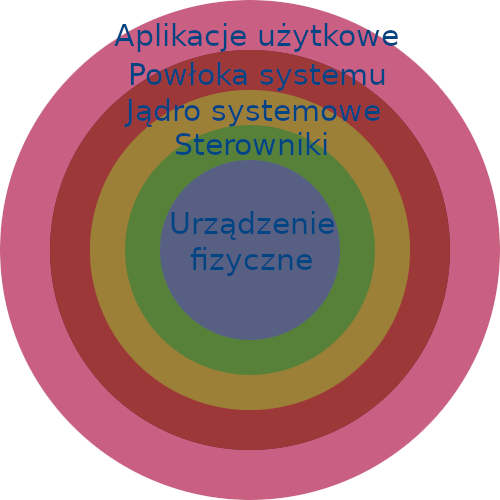
\includegraphics[height=100mm]{schemat_os.png}
%	\captionof{figure}{Schmat warstw systemu operacyjnego}
%\end{center}

Plan pracy jest następujący. W części teortycznej zostaną omówione mechanizmy stojące za działaniem maszyn wirtualnych i konterów na platformie docker oraz ich porównanie. Natępnie omówiony zostanie schemat wdrożenia aplikacji. Część praktyczna będzie zawierać szczegółowy opis przygotowania środowiska oraz wdrożenia aplikacji zarówno przykładowych jak i tych pochodzących z wydziałowego systemu informatycznego. 

\section{Założenia projektu}
Celem projektowej części pracy jest opracowanie skalowalnego środowiska usług internetowych, działającego w oparciu o technologię kontenerów Docker na platformie Linux w systemie wirtualizacji VMware ESX. Usługi realizowane przez system mają obejmować obsługę: - internetowych serwisów aplikacyjnych działających w technologiach odpowiednio: PHP, Apache Tomcat, Python Django, - witryn CMS WordPress, - serwerów relacyjnych baz danych MySQL, PostgreSQL. Elementem pracy będzie także migracja istniejących serwisów internetowych do ich odpowiadających im instancji wyżej wymienionych kontenerów Docker oraz ocena uzyskanych korzyści pod kątem konsumowanych zasobów sprzętowych i wydajności działania. 

\chapter{Podstawa Teoretyczna}
\section{Wirtualizacja}
Szeroko rozumiane urządznie zwane komputerem składa się z dwóch kategorii komponentów: urządzeń fizycznych i oprogramowania. W skład urządzeń fizycznych wchodzą między innymi płyta główna, centralna jednostka przetwarzająca i urządzenia wejścia/wyjścia. Oprogramowanie składa się z warstw, najniżej, najbliżej sprzętu znajduje się oprogramownie do zarządzania i komunikacji z urządzaniami, w wyższych warstwach znajdziemy aplikacje użytkowe. Zadaniem systemu operacyjnego jest zarządzanie zarówno zasobami sprzętowymi jak i oprogramowaniem. Stanowi on interfejs pomiędzy maszyną a użytkownikem, umożliwiając tym samym stosowanie komputerów do celów osobistych znanych nam z życia codziennego i profesjonalnych na linii człowiek - maszyna, ale i maszyna - maszyna. Ideą stojącą za systemem operacyjnym jest istnienie środowiska, które dynamicznie będzie tłumaczyć zlecenia użytkownika na język maszynowy, następnie zlecać sprzętowi ich wykonanie i w drugą stronę poinformować użytkownia o rezultatach pracy maszyny oraz jej zapotrzebowaniach na dane, zachowując jednocześnie optymalne działanie pracy całego systemu i zawartych w nim urządzeń.
   
\begin{center}
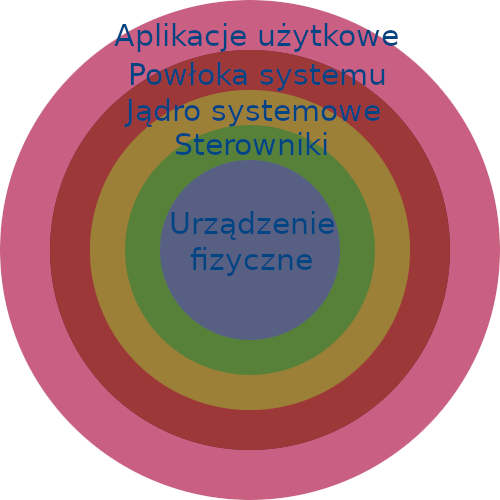
\includegraphics[height=100mm]{schemat_os.png}
\captionof{figure}{Schmat warstw systemu operacyjnego}
\end{center}

Na powyższym rysunku 2.1 przedstawiony jest schemat budowy systemu oparecyjnego. W skład samego systemu opracyjnego wchodzą sterowniki, jądro i powłoki systemowe. System operacyjny jest również podzielony na przestrzenie jądra i użytkownika. Wirtualizacja zatem jest symulacją warstwy fizycznej komputera na której można zainstalować i używać dowolnego systemu operacyjnego. Zasymulować można różnego rodzaju architektury i parametry sprzętowe, zalecane jest jednak by wirtualna platforma sprzętowa nie przekraczała możliwości rzeczywistego sprzętu. Wirtualizacji można dokonać na kilku poziomach. 
\subsection {Poziom architektury zestawu instrukcji (ISA)}
Tak zwana pełna wirtualizacja. Wszytkie instrukcje procesorowe systemu gościa są interpretowane przez emulator, a następnie mapowane na rzeczywisty sprzęt fizyczny gospodarza. Dalej instrukcje są wykonywane i zwracane do emulatora kóry przekazuje je do gościa. Z racji długiej drogi jaką musi pokonać pojendyczna instrukcja to rozwiązanie należy do najwolniejszych. Tą metode stosuje się, gdy architektury sprzętowe gościa i gospodarza są zbyt różne, aby dało się je zmapować lub jest to nieopłacalnie trudne. Rozwiąnie to stosuję się na przykład do emaluacji środowisk smartfonów, konsol do gier i mikrokontrolerów.
\subsection {Poziom warstwy abstrakcji sprzętowej (HAL)}
Inaczej nazywany poziomem sprzętowego wspomagania. Ta metoda wirtulizacji polega na mapowaniu rzeczywistych zasobów sprzętowych na wirtualne zasoby. Zatem wszystkie instrukcje nieuprzywilejowane są wykonywane bezpośrednio na sprzęcie gospodarza. Instrukcje uprzywilejowane, czyli takie które może wykonać tylko gospodarz są przekazywane do hipernadzorcy i ten je wykonuje. Rozwiąznie to jest zasadniczo szybsze od wirtualizacji zestawu instrukcji. Z tej metody korzystają narzędzia do wirtualizacji takie jak VMWare Workstation, Oracle VirtualBox i wiele innych.
\subsection {Poziom systemu operacyjnego}
Wirtualizacja na poziomie systemu opercyjnego pozwala na działanie kilku odrębnych odizolowanych od siebie systemów operacyjnych, a dokładnie przestrzeni użytkownia korzystających z jednego jądra systemowego. Co za tym idzie nie dochodzi do duplikacji całych systemów operacyjnych i co za tym idzie nie jest wymagana praca hipernadzorcy. Rozwiązanie takie jest nazywane konteneryzacją i jest stosowane na takich platformach jak Docker, CoreOS, LXC i Oracle Solaris Containers. Wadą tej metody jest przymus używania tylko takich systemów operacyjnych, które mogą współdzielić jądro z systemem gospodarza. Nic jednak nie stoi na przeszkodzie aby umieścić kontenery na maszynie wirtualnej postawionej na poziomie wspierania sprzętowego, jednak spowolni to szybkość tych kontenerów do szybkości samej maszyny wirtualnej. 
\subsection {Poziom bibliotek lub języków programownia}
Stosowane w ramach technologii JIT (just in time). Niektóre środowiska programistyczne pozwalają na kompilację kodu źródłowego do postaci kodu pośredniego, który nie ma bezpośredniego przełożenia na kod maszynowy. Program jest wykonywany na maszynie wirtualnej, która kompiluje kod pośredni do kodu maszynowego, a może to zrobić zarówno na poczatku wywołania programu lub pierwszego wywołania konkretnej części kodu. Z tej technologii korzysta Java, .Net, Python i wiele innych języków programowania. 
\subsection {Poziom aplikacji}
Wirtualizowane są tylko aplikacje, co oznacza, że nie wykorzystują one bezpośrednio dostarczanego przez system operacyjny środowiska wykonawczego, a używją dostarczonego przez inna aplikacje takie środowisko na jakie zostały zbudowane. Przykłądem platformy umożliwijącej wirtualizacje aplikacji jest Wine, która umożliwia działanie aplikacji przystowanych do pracy w systemie MS Windows na systemie operacyjnym typu Linux.
 
\section{Hipernadzorca}
Komponentem systemu komputerowego umożliwiającym dokonanie wirtualizacji na poziomie wsparcia sprzętowego jest hipernadzorca (hypervisor). Rozróżnanie są dwa typy hipernadzorców:

\subsection {Hipernadzorca typu pierwszego} 
Tak zwany hipernadzorca natywny (bare metal) osadzony bezpośrednio na sprzęcie nie wymaga zainstalowanego systemu operacyjnego gospodarza. Pozwala on osadzać maszyny wirtualne nad sobą co znacząco upraszca schemat abstrakcji architektury całego systemu. Przykładami tego typu hipernadzorców są MS Hyper-V i VMWare ESXi.
%\begin{center}
%	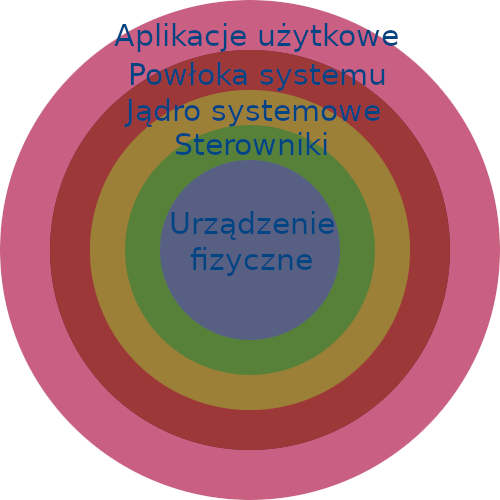
\includegraphics[height=100mm]{schemat_os.png}
%	\captionof{figure}{Schmat warstw systemu operacyjnego}
%\end{center}

\subsection {Hipernadzorca typu drugiego} 
Hipernadzorca hostowany jest osadzony w systemie operacyjnym gospodarza jako aplikacja. Takimi aplikacjami są przykłądowo VMWare Workstation, VMWare Player, VirtualBox i QEMU.
%\begin{center}
%	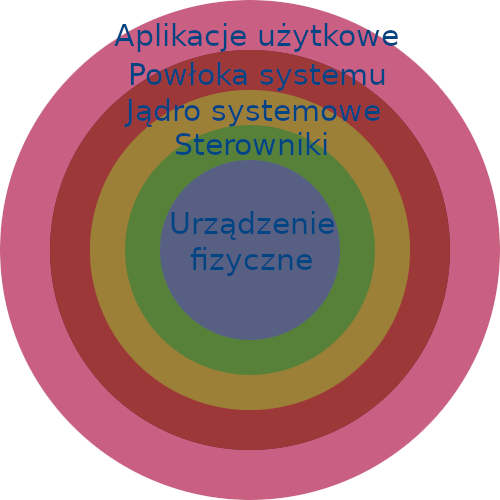
\includegraphics[height=100mm]{schemat_os.png}
%	\captionof{figure}{Schmat warstw systemu operacyjnego}
%\end{center}

\section{Konteneryzacja}
Konteneryzacja jako wirtualizacja na poziomie systemu opercyjnego z racji wspóldzielenia przez kontenery jądra systemu gospodarza powinna cechować większą wydajnością od wirtulizacji na poziomie ISA lub HAL. O ile nie zastąpi ona klasycznych maszyn wirtualnych pod względem możliowści uruchamiania różnorodnych systemów operacyjnych, a tyle najmocniejszą stroną konteneryzacji jest dużo niższe zapotrzebowanie na pamięć twardą, co za tym idzie przenaszalność oraz szybkość zarówno działania jak i startowania. Współdzielenie jądra systemowego oraz dostępu do fizycznej warstwy komputera niesie ze sobą pewne ryzyko jakim jest drastyczny spadek wydajności. Wszystkie kontenery konkurują ze sobą o zasoby sprzętowe, ale również o zasoby jądra. Jądro systemu jest bardzo skomplikowanym oprogramowaniem. Zdaża się, że zbyt obciążone przez kontenery jądro znacząco spowolni, a w konsekwncji utworzy szyjke od butelki (bottle neck) pomiędzy warstwami użytkownika i warstwą fizyczną.   

%\begin{center}
%	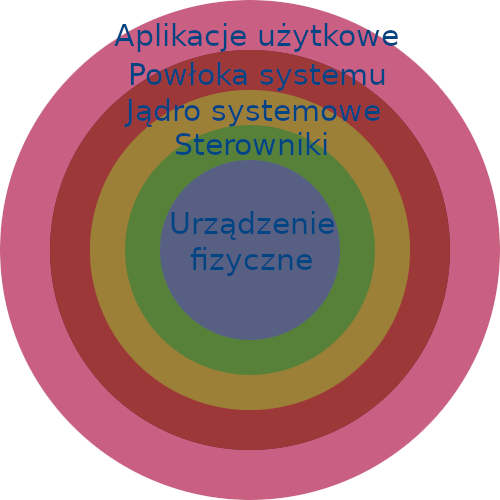
\includegraphics[height=100mm]{schemat_os.png}
%	\captionof{figure}{Schmat warstw systemu operacyjnego}
%\end{center}

\chapter{Założenia projektowe}
\section{Architektura wejściowa serwisów}
\subsection{Platforma systemu serwerowego}
Na wydziałowym serwerze zainstalowny jest hipernadzorca typu pierwszego, dokładnie VMWare ESX, osadzony bezpośrednio nad warstwą fizyczną klastra komputerowego. Na serwerze wdrożonych jest szereg aplikacji działających na odrębnych maszynach wirtulanych. 

\subsection {Wizualizaja platformy wejściowej} Na poniższym rysunku znajduje się schemat wejściowej architektury systemu serwerowego, który w ramach tej pracy ma zostać przekształcony.
%\begin{center}
%	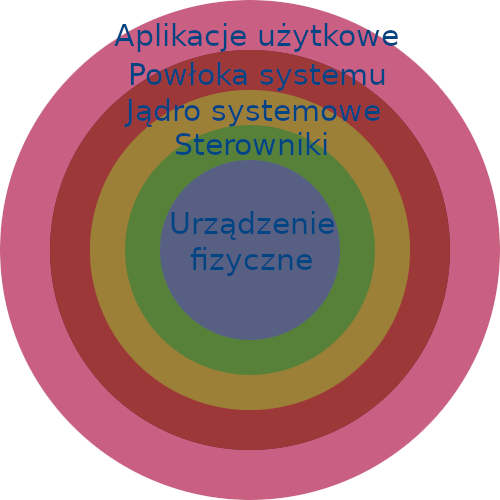
\includegraphics[height=100mm]{schemat_os.png}
%	\captionof{figure}{Schmat warstw systemu operacyjnego}
%\end{center}

\section{Architektura docelowa serwisów}
Koncepcja architektury docelowej jest zlikwidowanie pewnej ilości maszyn wirtulanych i przeniesienie serwisów w nich zawartych do kontenerów znajdujących się w jednej maszynie wirtualnej. Oczywistą korzyścią z tej akcji jest zaoszczędzenie pewnej, być może nawet dużej ilości  pamięci twardej. Nie jest jednak oczywiste do jakiej zmiany dojdzie w kwestii wydajonści. O ile pierwotny układ składa się z jednego poziomu wirtualizacji, tak ten układ będzie się składał z dwóch: wirtualizacji wspomaganej sprzętowo oraz na poziomie systemu oparcyjnego.
%\begin{center}
%	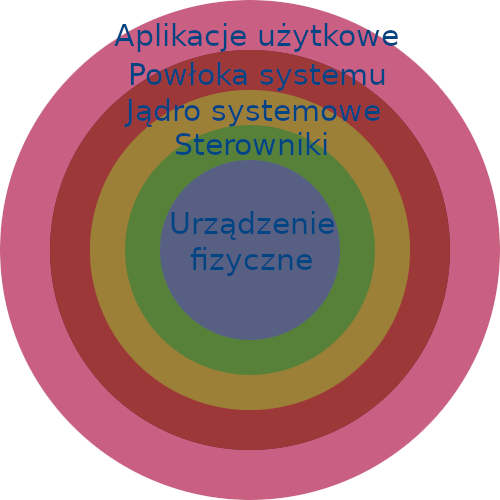
\includegraphics[height=100mm]{schemat_os.png}
%	\captionof{figure}{Schmat warstw systemu operacyjnego}
%\end{center}

\chapter{Opis przykładowych aplikacji i ich wdrożenie}
\section{Opis}
Przykładowe aplikacje to najprostsze aplikcję o identycznych wymaganiach jak aplikację pochodzące z wydziałwego serwera. Aplikacja java spring boot jest naprostszym serwisem http wyświetlający prostą zawartość w przegląderce internetowej. Serwis apache-php również jest serwisem http, który udostępnia przez przeglądarkę interfejs CRUD do trzeciego serwisu, który dostarcza bazę danych PostgreSQL.  
\section{Środowisko projektowe i wymagania aplikacji}
\subsubsection{Środowisko projektowe:}
\begin{itemize}[noitemsep]
    \item Narzędzie do wirtualizcji VMWare Workstation Player 15.5
    \item System operacyjny Debian 10.2
    \item Docker 19.03.5
    \item Docker-compose 1.25.0
\end{itemize}

\subsubsection{Wymagania Aplikacji:}
\begin{itemize}[noitemsep]
    \item Apliakcja Java Spring Boot
    \begin{itemize}[noitemsep]
    	\item Java 8 lub nowsza
    \end{itemize}
    \item Aplikacja php
	\begin{itemize}[noitemsep]
		\item php 5.4 lub nowsze z dodatkiem umożliwiającym połączenie z bazą danych PostgreSQL
		\item Apache 2 lub nowszy
		\item Dostęp do istniejącej bazy danych PostgreSQL
	\end{itemize}
\end{itemize}

\section{Działanie i powiązania zbioru konenerów}
\subsubsection{Docker}
Platforma Docker do utowrzenia kontenera wymaga dwóch komponentów zbudowanej aplikacji i jej zasóbów w postacji na przykład plików html, skryptów itd. oraz pliku konfiguracyjnego dockerfile na podstawie którego zostanie utworzona przestrzeń użytkownika w kontenerze. Wykorzystanymi komendami dockerfile w projekcie są:
\begin{itemize}[noitemsep]
	\item RUN wykonuję polecnie powłoki systemu operacyjnego w konenerze podczas jego budowy
	\item CMD nadpisuje domyślną instrukcje 'command', która domyślnie uruchamia aplikacje wewnątrz kontenera. Dotyczy to przypadku w którym kontener pracuje w trybie odłączonym od powłoki systemu gospodarza. Instrukcja CMD może zostać wykorzystana raz, każda kolejna nadpisze poprzednią, w konsekwencji wykonana zostanie tylko ostatnia.
	\item COPY kopiuje pod podane miejsce w systemie plików gościa wskazane pliki i katalogi z systemu plików gospodarza
	\item ADD jest to rozszerzona instrukcja COPY, pozwala również dodać plików z pod podanego adresu url oraz automatycznie rozpakować foldery skompresowane w trakcie kopiowania
	\item ENTRYPOINT wykonuje tę samą czynność co CMD z tą różnicą, że może być użyta wielokrotnie i każde użycie zostanie wykonane. Instrukcje ENTRYPOINT i CMD nie kolidują ze sobą
	\item VOLUME tworzy obszar w pamięci w którym będzie przechowywana kopia danych wygenerownych przez kontener, np. logi, bazy danych itd.
	\item FROM instrukcja której obecność jest zawsze wymagana do zbudowania obrazu. Musi znajdować się w pierwszej linii pliku docker file. Jej argumentem jest tag obrazu który ma zostać zbudowny. W trakcie budowy obraz jest pobierany z repozytorium.
	\item ENV tworzy zmienna środowiskową w goszczonym systemie opercyjnym
	\item EXPOSE pokazuje port widoczny dla maszyn zewnętrznych
\end{itemize}
Z racji tego, iż wybranym system opercyjnym gospodarza dla konteneróW jest Debian 10, dockerfile musi zawierać komendy która zainstaluje wymagane do działania aplikacji paczki i biblioteki oraz koniecznie korzystać z obrazów systemów z rodziny Linux. Musi również zawierać
\subsubsection{Docker-compose}
W przypadku kiedy w systemie pracuje wiele kontenerów pojawia się problem zarządzania nimi. Uruchamianie każdego kontenera z wiersza poleceń jest żmudnym i podatnym na pomyłki procesem. Zastosowanie skryptu np. w powłoce bash cechowałoby się nie małą nieprzerzystością. Programem służącym do tego celu jest Docker-compose. Pozwala on budowanie i uruchamianie wielu kontenerów docker jednocześnie. Tak jak Docker, Docker-compose wymaga pliku konfiguracyjnego, tym razem w notacji YAML i o rozszerzeniu docker-compose.yml. W tym pliku są zawarte lokacje plików dockerfile i parametry służące do budowy i uruchomienia obrazu oraz konfiguracja sterowników np. sieciowych. 
\subsubsection{Aplikacja Java spring boot}
Realizuje najprostsze zadanie. Wyświetla "Hell World!"
\subsubsection{Aplikacja php}

\subsubsection{Baza danych PostgreSQL}

\section{Zrealizowane pliki dockerfile}

\chapter{Wdrożenie rzeczywistych serwisów wydziałowego systemu informatycznego}

\chapter{Wnioski}

\chapter{Kod źródłowy}
\section{Repozytorium Git}
\section{Dołączona płyta CD}

\chapter{Bibliografia}

\end{document}